
\documentclass[border=10pt, tikz]{standalone}
\usepackage{xcolor}

\definecolor{StemColor}{RGB}{255,235,59}
\definecolor{BlockColor}{RGB}{255,193,7}
\definecolor{DownColor}{RGB}{255,152,0}
\definecolor{PoolColor}{RGB}{121,85,72}

\usetikzlibrary{positioning, shapes, arrows.meta, fit}

\begin{document}
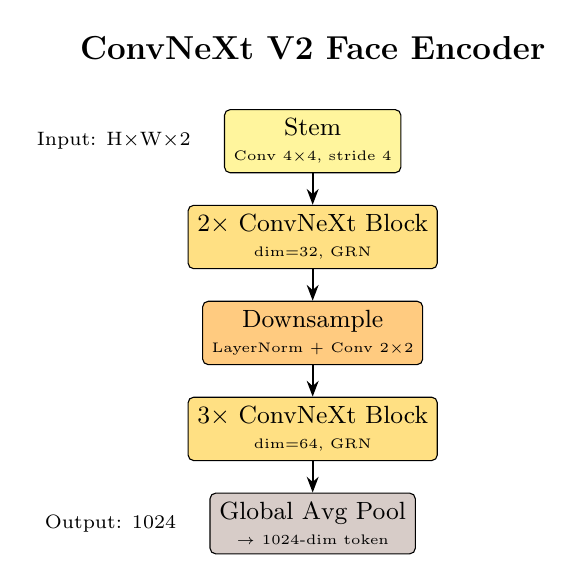
\begin{tikzpicture}[
    node distance=0.5cm,
    block/.style={rectangle, draw, rounded corners=2pt, minimum height=0.7cm, minimum width=2cm, align=center, font=\small},
    arrow/.style={-{Stealth[length=2mm]}, thick},
]

% Title
\node[font=\large\bfseries] (title) {ConvNeXt V2 Face Encoder};

% Stem
\node[block, fill=StemColor!50, below=0.5cm of title] (stem) {
    Stem\\[-2pt]
    \tiny Conv 4$\times$4, stride 4
};

% Block 1
\node[block, fill=BlockColor!50, below=0.4cm of stem] (block1) {
    2$\times$ ConvNeXt Block\\[-2pt]
    \tiny dim=32, GRN
};

% Downsample
\node[block, fill=DownColor!50, below=0.4cm of block1] (down) {
    Downsample\\[-2pt]
    \tiny LayerNorm + Conv 2$\times$2
};

% Block 2
\node[block, fill=BlockColor!50, below=0.4cm of down] (block2) {
    3$\times$ ConvNeXt Block\\[-2pt]
    \tiny dim=64, GRN
};

% Global Pool
\node[block, fill=PoolColor!30, below=0.4cm of block2] (pool) {
    Global Avg Pool\\[-2pt]
    \tiny $\rightarrow$ 1024-dim token
};

% Arrows
\draw[arrow] (stem) -- (block1);
\draw[arrow] (block1) -- (down);
\draw[arrow] (down) -- (block2);
\draw[arrow] (block2) -- (pool);

% Input/Output labels
\node[left=0.3cm of stem, font=\scriptsize] {Input: H$\times$W$\times$2};
\node[left=0.3cm of pool, font=\scriptsize] {Output: 1024};

\end{tikzpicture}
\end{document}
